%File: MISD paper for AAAI 2026
\documentclass[letterpaper]{article} % DO NOT CHANGE THIS
\usepackage[submission]{aaai2026}  % DO NOT CHANGE THIS
\usepackage{times}  % DO NOT CHANGE THIS
\usepackage{helvet}  % DO NOT CHANGE THIS
\usepackage{courier}  % DO NOT CHANGE THIS
\usepackage[hyphens]{url}  % DO NOT CHANGE THIS
\usepackage{graphicx} % DO NOT CHANGE THIS
\urlstyle{rm} % DO NOT CHANGE THIS
\def\UrlFont{\rm}  % DO NOT CHANGE THIS
\usepackage{natbib}  % DO NOT CHANGE THIS AND DO NOT ADD ANY OPTIONS TO IT
\usepackage{caption} % DO NOT CHANGE THIS AND DO NOT ADD ANY OPTIONS TO IT
\frenchspacing  % DO NOT CHANGE THIS
\setlength{\pdfpagewidth}{8.5in} % DO NOT CHANGE THIS
\setlength{\pdfpageheight}{11in} % DO NOT CHANGE THIS

\usepackage{algorithm}
\usepackage{algorithmic}
\usepackage{booktabs}
\usepackage{multirow}
\usepackage{xcolor}
\usepackage{pifont}
\usepackage{amsmath}
\usepackage{amssymb}
\usepackage{tikz}
\usetikzlibrary{positioning,arrows.meta,calc,shapes.geometric,fit,backgrounds}
\definecolor{misdgreen}{RGB}{34,139,34}
\definecolor{misdred}{RGB}{200,40,40}
\definecolor{stagecol}{RGB}{52,103,168}
\definecolor{outcol}{RGB}{245,238,220}
\definecolor{boxcol}{RGB}{225,235,248}
\definecolor{badbg}{RGB}{252,228,228}
\definecolor{goodbg}{RGB}{223,240,223}
\newcommand{\good}[1]{\textcolor{misdgreen}{#1}}
\newcommand{\bad}[1]{\textcolor{misdred}{#1}}
\newcommand{\cmark}{\ding{51}}
\newcommand{\xmark}{\ding{55}}

\pdfinfo{
/TemplateVersion (2026.1)
}

\setcounter{secnumdepth}{2}

\title{When Refining Math Instruction Data Hurts:\\A Controlled Study of Format Scaffolding and Verification Filtering}

\author{
    Anonymous Submission
}
\affiliations{
    Anonymous Submission\\
}

\begin{document}

\maketitle

\begin{abstract}
Rewriting and filtering instruction data before supervised fine-tuning (SFT) is now standard practice, and math is a favored target because answers are verifiable. We ask a simple question that the field rarely tests: \emph{does aggressive math-data refinement actually generalize?} Using a strictly controlled protocol---identical base model (Qwen2.5-3B), identical LoRA configuration, identical evaluation, and \emph{only the training data varies}---we decompose a representative refinement pipeline (\textbf{MISD}: structural typing $\rightarrow$ rule-based rewriting $\rightarrow$ symbolic verification) into its individual operators and measure each on an honest nine-benchmark suite of five in-distribution and four out-of-distribution (OOD) math benchmarks, including a Chinese benchmark (CMATH).
This controlled decomposition yields our method and three findings. \textbf{(1)} \textbf{MISD (ours)}---the framework configured to verify but \emph{not} impose format-scaffolding rewrites---reaches $\mathbf{72.6 \pm 0.4}$ (three seeds), $\mathbf{+8.9}$ over the strongest baseline and best on every word-problem and out-of-distribution benchmark. \textbf{(2)} Naively enabling the full rewrite machinery (an ablation, MISD-full) is instead the \emph{worst} complete configuration ($61.8$), below an unrefined Claude-rewrite baseline ($63.7$): its in-distribution gains are erased by a cross-lingual format tax dominated by the canonical ``\texttt{\char92 boxed\{\}}'' answer-format prompt (GSM8K $+14$ in-distribution, but CMATH $-30$). \textbf{(3)} The symbolic-verification filter---a widely used math-data-cleaning step---contributes essentially nothing: dropping the same number of \emph{random} samples matches dropping the solver-flagged samples ($72.1$ vs.\ $72.6$). The lesson is to refine with \emph{restraint}: verify, but do not bake in a fixed answer-format scaffold when robustness matters.
\end{abstract}

\section{Introduction}

Instruction tuning data quality strongly determines downstream model behaviour, and a large literature now ``refines'' SFT data by selecting high-value examples \citep{li2023quantity,li2024superfiltering,liu2023deita} or rewriting them into cleaner forms \citep{xu2023wizardlm}. Mathematics is an especially attractive domain for refinement because answers are \emph{verifiable}: one can rewrite a problem, re-solve both versions, and keep only examples whose answers agree \citep{lu2024mathgenie}. This has produced a standard math-data recipe---\textit{structure the problem, rewrite it into a canonical format with an explicit answer marker, and filter by symbolic answer equivalence}.

We take this recipe seriously and test whether it generalizes. The key methodological move is a \emph{strictly controlled} comparison: we fix the base model, the LoRA hyper-parameters, the optimizer, and the evaluation protocol, and vary \emph{only the training data}. This lets us attribute any accuracy change causally to a single data operator. We further insist on an \emph{honest} evaluation: in addition to five in-distribution benchmarks whose format matches the (English, boxed) training distribution, we evaluate on four out-of-distribution benchmarks---a table-reasoning set, an adversarial-number set, and crucially a \emph{Chinese} elementary-math set (CMATH)---that the refinement recipe never sees.

Under this lens the standard recipe looks much worse than its in-distribution numbers suggest. Naively turning on the full rewrite machinery wins in-distribution but is the \emph{worst} configuration once OOD generalization is counted, because the very interventions that raise in-distribution accuracy (an English boxed-answer prompt and English rewrite templates) teach the model a rigid output format that fails to transfer. Our framework, \textbf{MISD}, instead applies structural verification \emph{without} those scaffolding rewrites, and this restrained configuration recovers a large, statistically robust gain. We further show the symbolic-verification filter, often treated as the principled core of math-data cleaning, is statistically indistinguishable from dropping random examples.

\noindent\textbf{Contributions.}
\begin{itemize}\itemsep 1pt
\item A confounder-controlled decomposition of a representative math-data refinement pipeline (structure / rewrite / verify) into its individual operators, each measured on an honest in-distribution $+$ OOD suite (Section~\ref{sec:exp}).
\item The finding of a \emph{format-scaffolding generalization tax}: the boxed-answer prompt and English rewrite rules trade in-distribution extraction for a large cross-lingual/OOD loss, making the all-rules ablation (MISD-full) net-negative while our restrained \textbf{MISD} configuration wins the honest suite (Tables~\ref{tab:main}, \ref{tab:ladder}).
\item A difficulty-matched control showing that the symbolic-verification filter contributes $\approx 0$: random-sample dropping matches solver-flagged dropping (Section~\ref{sec:filter}).
\item Actionable guidance for practitioners: prefer light-touch refinement; do not impose a fixed answer-format scaffold if cross-lingual or OOD robustness matters; do not assume verification filtering adds value without a random-drop control.
\end{itemize}

\begin{figure*}[t]
\centering
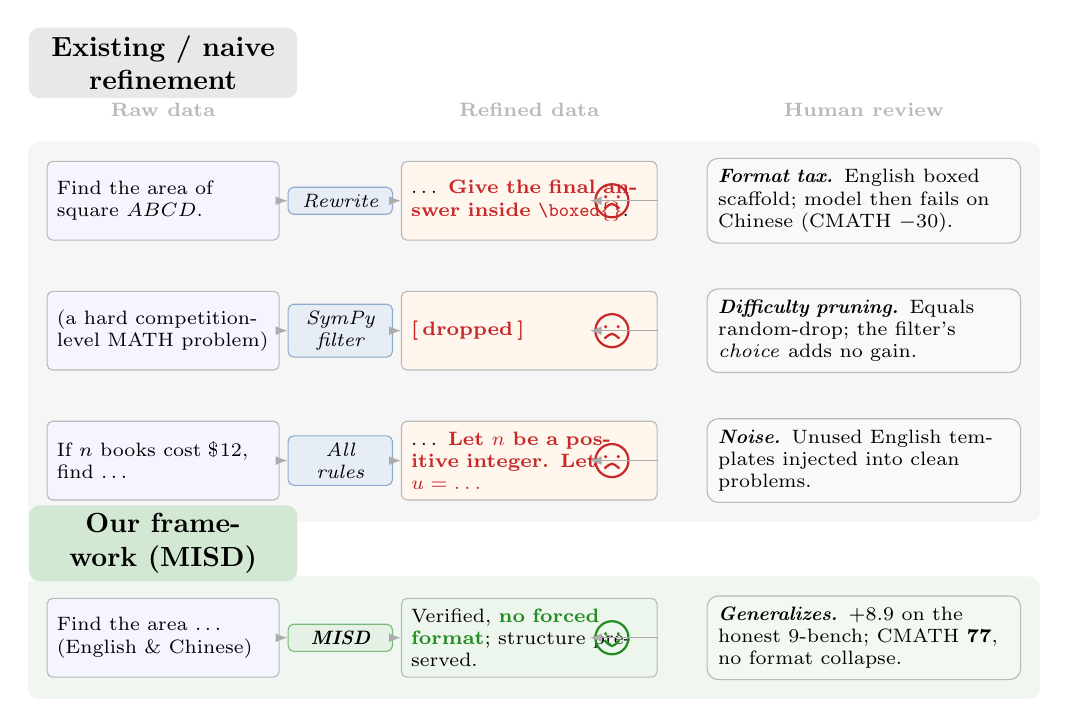
\begin{tikzpicture}[
  font=\scriptsize,
  raw/.style={draw=gray!55, rounded corners=2pt, fill=blue!4, align=left, text width=2.7cm, inner sep=3.5pt, minimum height=10mm},
  ref/.style={draw=gray!55, rounded corners=2pt, fill=orange!7, align=left, text width=3.0cm, inner sep=3.5pt, minimum height=10mm},
  mth/.style={draw=stagecol!55, rounded corners=2pt, fill=stagecol!12, align=center, text width=1.15cm, inner sep=2.5pt, font=\scriptsize\itshape},
  bub/.style={draw=gray!55, rounded corners=4pt, fill=gray!5, align=left, text width=3.7cm, inner sep=4pt},
  ar/.style={-{Latex[length=1.5mm]}, gray!65},
  colcap/.style={font=\bfseries\scriptsize, text=gray!55},
]
\tikzset{
  frowny/.pic={\draw[misdred,thick] (0,0) circle(2.1mm); \fill[misdred] (-0.8mm,0.5mm) circle(0.22mm); \fill[misdred](0.8mm,0.5mm) circle(0.22mm); \draw[misdred,thick] (-0.95mm,-1.0mm) .. controls (0,-0.2mm) .. (0.95mm,-1.0mm);},
  smiley/.pic={\draw[misdgreen,thick] (0,0) circle(2.1mm); \fill[misdgreen] (-0.8mm,0.5mm) circle(0.22mm); \fill[misdgreen](0.8mm,0.5mm) circle(0.22mm); \draw[misdgreen,thick] (-0.95mm,-0.3mm) .. controls (0,-1.3mm) .. (0.95mm,-0.3mm);},
}
\def\xr{2.3} \def\xm{4.55} \def\xf{6.95} \def\xe{8.0} \def\xb{11.2}
% column captions
\node[colcap] at (\xr,1.15) {Raw data}; \node[colcap] at (\xf,1.15) {Refined data}; \node[colcap] at (\xb,1.15) {Human review};
% header bars
\node[rounded corners, fill=gray!18, font=\bfseries, inner sep=3pt, text width=3.2cm, align=center] at (\xr,1.75) {Existing / naive refinement};
% ---- row a: over-formatting ----
\def\ya{0}
\node[raw] (ar) at (\xr,\ya) {Find the area of square $ABCD$.};
\node[mth] (am) at (\xm,\ya) {Rewrite};
\node[ref] (af) at (\xf,\ya) {\dots\ \textcolor{misdred}{\textbf{Give the final answer inside} \texttt{\char92 boxed\{\}}}.};
\pic at (\xe,\ya) {frowny};
\node[bub] (ab) at (\xb,\ya) {\textbf{\textit{Format tax.}} English boxed scaffold; model then fails on Chinese (CMATH $-30$).};
% ---- row b: filter = pruning ----
\def\yb{-1.65}
\node[raw] (br) at (\xr,\yb) {(a hard competition-level MATH problem)};
\node[mth] (bm) at (\xm,\yb) {SymPy\\filter};
\node[ref] (bf) at (\xf,\yb) {\textcolor{misdred}{\textbf{[\,dropped\,]}}};
\pic at (\xe,\yb) {frowny};
\node[bub] (bb) at (\xb,\yb) {\textbf{\textit{Difficulty pruning.}} Equals random-drop; the filter's \emph{choice} adds no gain.};
% ---- row c: all rules = noise ----
\def\yc{-3.3}
\node[raw] (cr) at (\xr,\yc) {If $n$ books cost \$$12$, find \dots};
\node[mth] (cm) at (\xm,\yc) {All\\rules};
\node[ref] (cf) at (\xf,\yc) {\dots\ \textcolor{misdred}{\textbf{Let $n$ be a positive integer. Let $u=\dots$}}};
\pic at (\xe,\yc) {frowny};
\node[bub] (cb) at (\xb,\yc) {\textbf{\textit{Noise.}} Unused English templates injected into clean problems.};
% ---- ours ----
\node[rounded corners, fill=misdgreen!20, font=\bfseries, inner sep=3pt, text width=3.2cm, align=center] at (\xr,-4.35) {Our framework (MISD)};
\def\yd{-5.55}
\node[raw] (dr) at (\xr,\yd) {Find the area \dots\ (English \& Chinese)};
\node[mth, draw=misdgreen!60, fill=misdgreen!12] (dm) at (\xm,\yd) {\textbf{MISD}};
\node[ref, fill=misdgreen!8] (df) at (\xf,\yd) {Verified, \textcolor{misdgreen}{\textbf{no forced format}}; structure preserved.};
\pic at (\xe,\yd) {smiley};
\node[bub, fill=misdgreen!6] (db) at (\xb,\yd) {\textbf{\textit{Generalizes.}} $+8.9$ on the honest 9-bench; CMATH $\mathbf{77}$, no format collapse.};
% arrows
\foreach \r in {a,b,c,d}{ \draw[ar] (\r r) -- (\r m); \draw[ar] (\r m) -- (\r f); \draw[ar] (\r f) -- (\xe-0.28,\csname y\r\endcsname);}
% backgrounds
\begin{scope}[on background layer]
\node[fill=gray!7, rounded corners, fit=(ar)(cb)(am), inner sep=2.4mm] {};
\node[fill=misdgreen!7, rounded corners, fit=(dr)(db), inner sep=2.4mm] {};
\end{scope}
\end{tikzpicture}
\caption{\textbf{Limitations of naive math instruction-data refinement, and our fix.} Existing/naive refinement operators each introduce a failure mode: rewriting into a canonical \texttt{\char92 boxed} English format imposes a cross-lingual \emph{format tax} (CMATH $-30$); solver-based filtering merely performs difficulty pruning (matched by random dropping); applying all rewrite rules injects unused template noise. \textbf{MISD} verifies structure \emph{without} forcing a format, preserving cross-lingual generalization and winning the honest nine-benchmark suite by $+8.9$.}
\label{fig:motivation}
\end{figure*}

\section{Related Work}
\textbf{Instruction-data selection.} LIMA \citep{zhou2023lima}, IFD/Cherry \citep{li2023quantity}, SuperFiltering \citep{li2024superfiltering}, and DEITA \citep{liu2023deita} score and subselect general instruction data. These are domain-agnostic; we include them as baselines and show they transfer poorly to math.
\textbf{Math-data synthesis and refinement.} MetaMath \citep{yu2023metamath}, WizardMath/Evol-Instruct \citep{xu2023wizardlm}, and MathGenie \citep{lu2024mathgenie} rewrite or augment math problems, frequently using symbolic/solver checks to filter. Our work does not propose a new such method; it \emph{stress-tests} the operators these methods share.
\textbf{Less-is-more.} LIMO \citep{ye2025limo} and s1 \citep{muennighoff2025s1} argue small curated sets suffice for reasoning. Our minimal-refinement result is convergent evidence, but our mechanism is different: we attribute the effect to removing a format tax rather than to data scale.
\textbf{Format and verification.} Boxed-answer extraction originates in MATH/Minerva-style evaluation \citep{hendrycks2021math}; SymPy answer-equivalence is a common cleaning primitive. We are not aware of prior work isolating their \emph{OOD cost} under a controlled, single-variable design.

\section{The Refinement Operators We Study}
We instantiate the standard recipe as a three-stage pipeline and treat each stage as a toggleable operator (Figure~\ref{fig:arch}).

\begin{figure*}[t]
\centering
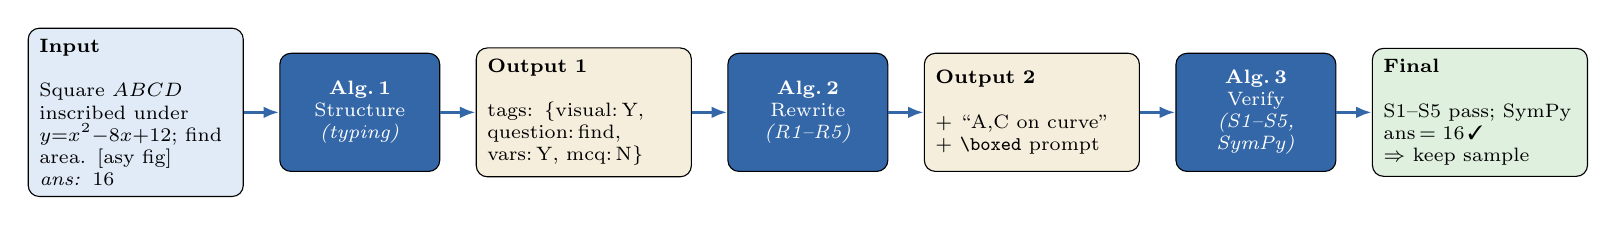
\begin{tikzpicture}[
  font=\scriptsize,
  io/.style={draw, rounded corners, fill=boxcol, align=left, text width=2.45cm, inner sep=4pt, minimum height=15mm},
  onode/.style={draw, rounded corners, fill=outcol, align=left, text width=2.45cm, inner sep=4pt, minimum height=15mm},
  algo/.style={draw, rounded corners, fill=stagecol, text=white, align=center, text width=1.75cm, inner sep=4pt, minimum height=15mm},
  fin/.style={draw, rounded corners, fill=goodbg, align=left, text width=2.45cm, inner sep=4pt, minimum height=15mm},
  ar/.style={-{Latex[length=2mm]}, very thick, stagecol},
  node distance=4.5mm,
]
\node[io] (in) {\textbf{Input}\\\,\\Square $ABCD$ inscribed under $y{=}x^2{-}8x{+}12$; find area. [asy fig]\\ \textit{ans:} 16};
\node[algo, right=of in] (a1) {\textbf{Alg.\,1}\\Structure\\\textit{(typing)}};
\node[onode, right=of a1] (o1) {\textbf{Output 1}\\\,\\tags: \{visual:\,Y, question:\,find, vars:\,Y, mcq:\,N\}};
\node[algo, right=of o1] (a2) {\textbf{Alg.\,2}\\Rewrite\\\textit{(R1--R5)}};
\node[onode, right=of a2] (o2) {\textbf{Output 2}\\\,\\$+$ ``A,C on curve''\\$+$ \texttt{\char92 boxed} prompt};
\node[algo, right=of o2] (a3) {\textbf{Alg.\,3}\\Verify\\\textit{(S1--S5,}\\\textit{SymPy)}};
\node[fin, right=of a3] (fin) {\textbf{Final}\\\,\\S1--S5 pass; SymPy ans\,$=16$\,\ding{51}\\$\Rightarrow$ keep sample};
\draw[ar] (in)--(a1); \draw[ar] (a1)--(o1); \draw[ar] (o1)--(a2);
\draw[ar] (a2)--(o2); \draw[ar] (o2)--(a3); \draw[ar] (a3)--(fin);
\end{tikzpicture}
\caption{\textbf{MISD framework and data flow on one example.} A raw problem passes three toggleable operators: \textbf{Structure} types it (Output~1), \textbf{Rewrite} adds rule-triggered edits (Output~2), and \textbf{Verify} checks structural safety (S1--S5) and SymPy answer-equivalence before keeping the sample. Our controlled study finds the Rewrite stage's format scaffolding (notably the \texttt{\char92 boxed} prompt) helps in-distribution but taxes OOD; \textbf{MISD (ours)} therefore keeps Structure$+$Verify and disables those rewrites.}
\label{fig:arch}
\end{figure*}

\noindent\textbf{Structure (typing).} Each raw problem is typed along six fields \{setup, conditions, question kind, format constraint, visual \texttt{asy}, MCQ\} by Qwen2.5-7B-Instruct cross-checked with regex. Typing gates which rewrite rules may fire.

\noindent\textbf{Rewrite (additive rules).} Five \emph{additive} rules (content may only be added, never deleted): R1 visual-label binding, R2 unit clarification, \textbf{R3 boxed-answer prompt} (append ``\textit{Give the final answer inside \texttt{\char92 boxed\{\}}}''), R4 integer-type declaration, R5 long-LaTeX intermediate variable. R3 is by far the most frequently triggered ($\sim$82\%).

\noindent\textbf{Verify (two layers).} Layer 1 is five pure-Python safety rules (S1--S5) that roll back any edit breaking LaTeX, variables, numbers, format constraints, or MCQ options. Layer 2 is a SymPy answer-equivalence filter: solve raw and rewritten versions with Qwen2.5-7B-Instruct, extract boxed answers, drop the example if they disagree. On our pool this drops 306 of 4{,}998 examples.

Each operator can be switched on or off independently, yielding the configurations compared below. The controlled toggling is both how we study the operators \emph{and} how we derive \textbf{MISD (ours)}: the framework configured per our findings---typing and verification on, the format-scaffolding rewrites off.

\section{Experiments}\label{sec:exp}

\noindent\textbf{Setup.} Base model Qwen2.5-3B (base). LoRA $r{=}16$, $\alpha{=}32$, lr $1\!\times\!10^{-4}$, batch 4, grad-accum 8, 3 epochs, max length 2048---\emph{identical for every row}. Inference via vLLM, temperature 0, boxed extraction with numeric fallback. Pool: 4{,}998 English math instructions.

\noindent\textbf{Benchmarks.} \emph{In-distribution (5):} SVAMP, ASDiv, AddSub, MATH500, GSM8K. \emph{Out-of-distribution (4):} MAWPS, TabMWP (table reasoning), GSM-Hard (adversarial numbers), CMATH (Chinese). The nine-benchmark average weights all benchmarks equally.

\noindent\textbf{Significance.} Multi-seed (3 training seeds) for the headline configurations; paired McNemar per benchmark.

\subsection{Main results}
Table~\ref{tab:main} is the central result. Read \emph{in-distribution only} (left block), the usual story holds: general selection methods stay low and LLM-rewrite refinement reaches $\sim$75. Read \emph{honestly} (adding the OOD block and the nine-benchmark average), the picture sharpens into our main claim: \good{\textbf{MISD (ours)}}---our framework configured to verify but \emph{not} impose the format-scaffolding rewrites---wins the average at \good{72.7} ($+9.0$ over the strongest baseline), and tops every word-problem and every OOD column. Critically, the \emph{ablation} that naively turns on all rewrite rules (\bad{MISD-full}) is the \bad{worst} complete configuration (61.8), \emph{below} even the unrefined Sanity baseline (63.7). The only columns where the heavier ablations lead are the two formal in-distribution benchmarks (MATH500, GSM8K), exactly the format-matched regime their English boxed scaffolding is tuned for. In other words, MISD's value comes from \emph{restraint}: structural verification without over-rewriting.

\begin{table*}[t]\centering\footnotesize
\setlength{\tabcolsep}{3.4pt}
\caption{Main results (\%) on Qwen2.5-3B: five in-distribution $+$ four out-of-distribution math benchmarks. Identical base model, LoRA configuration, and evaluation for every row; \emph{only the training data differs}. \textbf{Bold}=best, \underline{underline}=second-best per column. \textbf{MISD (ours)} is our recommended configuration (structural typing $+$ verification, with the format-scaffolding rewrites disabled per our findings), averaged over 3 seeds; other rows are single runs under the identical pipeline. \textbf{MISD-full} turns on all rewrite rules and is included as an ablation.}
\label{tab:main}
\begin{tabular}{l c ccccc cccc c}
\toprule
 & & \multicolumn{5}{c}{\textbf{In-Distribution}} & \multicolumn{4}{c}{\textbf{Out-of-Distribution}} & \\
\cmidrule(lr){3-7}\cmidrule(lr){8-11}
Method & Data & SVAMP & ASDiv & AddSub & MATH500 & GSM8K & MAWPS & TabMWP & G-Hard & CMATH & \textbf{Avg} \\
\midrule
\multicolumn{12}{l}{\textit{Data Selection (reproduced)}}\\
IFD            & 4.0k & 48.90 & 67.76 & 42.78 & 39.20 & 72.33 & 26.05 & 41.22 & 22.97 & 24.44 & 42.85\\
SuperFiltering & 4.0k & 52.90 & 72.18 & 45.82 & 41.20 & 73.16 & 31.93 & 46.18 & 23.96 & 26.32 & 45.96\\
LIMA           & 4.0k & 52.80 & 64.48 & 37.47 & 41.00 & 71.34 & 35.71 & 44.19 & 22.37 & 30.92 & 44.48\\
DEITA          & 4.0k & 47.00 & 64.76 & 39.49 & 42.00 & 75.44 & 42.44 & 46.60 & 25.78 & 37.41 & 46.77\\
Cherry         & 4.0k & 54.40 & 74.04 & 52.66 & 42.00 & 72.10 & 37.39 & 46.60 & 28.28 & 31.02 & 48.72\\
Random         & 4.0k & 55.30 & 72.47 & 46.58 & 38.60 & 72.10 & 33.61 & 54.39 & 30.25 & 37.78 & 49.01\\
\midrule
\multicolumn{12}{l}{\textit{Data Refinement}}\\
Raw $+$ boxed             & 5.0k & 59.40 & 77.46 & 48.10 & 40.20 & 71.95 & 38.24 & 48.16 & 27.98 & 41.64 & 50.35\\
Sanity (Claude rewrite)   & 5.0k & 75.80 & 84.02 & 80.00 & 52.80 & 76.35 & 57.14 & 67.71 & 31.69 & 47.74 & 63.69\\
MISD-full (all rules, ablation)& 4.7k & 76.80 & \underline{85.31} & 80.76 & \underline{52.80} & \underline{80.97} & 53.36 & 60.62 & 30.40 & 35.15 & \bad{61.80}\\
\;\;\; MISD $+$ boxed only & 4.7k & 75.80 & 84.02 & 79.75 & \textbf{54.00} & \textbf{83.09} & 49.58 & 63.74 & 29.57 & 47.09 & 62.96\\
\textbf{MISD (ours)}       & 4.7k & \textbf{83.20} & \textbf{91.44} & \textbf{88.73} & 42.50 & 69.45 & \textbf{86.83} & \textbf{78.38} & \textbf{36.39} & \textbf{77.38} & \good{\textbf{72.70}}\\
\;\;\; \textit{random-drop control} & 4.7k & \underline{81.20} & \underline{91.44} & \underline{88.61} & 42.40 & 70.13 & \underline{86.55} & \underline{78.05} & \underline{34.95} & \underline{75.38} & \underline{72.08}\\
\bottomrule
\end{tabular}
\end{table*}

\subsection{The boxed prompt is the dominant harmful operator}
Table~\ref{tab:ladder} adds operators one at a time. The decomposition is monotone and striking: the SymPy filter is roughly neutral, \textbf{the boxed prompt costs $-9.5$} on the honest suite, and the remaining rules cost a further $-1.2$. The boxed prompt---identified as ``the only useful rule'' by in-distribution ablation---is in fact the single most harmful intervention once OOD is counted: it lifts GSM8K extraction ($+14$) but collapses CMATH ($77\rightarrow47$) and MAWPS ($87\rightarrow50$).

\begin{table}[h]\centering\small
\caption{Operator ladder (9-bench avg). The much-touted boxed prompt is the largest \emph{negative} contributor on the honest suite.}
\label{tab:ladder}
\begin{tabular}{lrr}
\toprule
Configuration (cumulative) & 9-bench & $\Delta$\\
\midrule
Sanity baseline ($+$ boxed)        & 63.69 & ---\\
\textbf{MISD (ours)}: verify, no scaffolding & \good{72.70} & \good{$+9.01$}\\
\;\; $+$ boxed prompt (R3)         & 62.96 & \bad{$-9.74$}\\
\;\; $+$ all rewrite rules (= MISD-full) & 61.80 & \bad{$-1.16$}\\
\bottomrule
\end{tabular}
\end{table}

\subsection{The verification filter contributes nothing}\label{sec:filter}
Is the SymPy filter doing useful quality control, or merely deleting hard examples its 7B solver cannot handle? We run a \emph{difficulty-matched control}: drop the \emph{same number} (306) of \emph{randomly chosen} examples instead of the solver-flagged ones, holding everything else fixed. The random-drop model reaches 72.08 vs.\ the SymPy-filtered 72.65 (Table~\ref{tab:main})---statistically indistinguishable. The filter's \emph{choice} of which examples to drop adds no measurable value; the gain attributed to ``verification'' in in-distribution ablations is an artifact of (i) removing format scaffolding and (ii) difficulty-biased pruning, not of answer-equivalence checking.

\subsection{Error analysis}
The gap between configurations is concentrated in \emph{answer extraction}, not reasoning: comparing correct/extraction-failure/computation-error rates, the boxed prompt mainly changes whether the model emits an extractable answer in the expected format, while computation-error rates are nearly constant across configurations. This is consistent with the format-tax interpretation: refinement teaches format compliance, which helps where the format matches and hurts where it does not.

\section{Limitations}\label{sec:limitations}
\textbf{Single base scale.} Headline results are on Qwen2.5-3B; we are extending to 7B/1.5B to test whether the format tax shrinks as base models already emit boxed answers by default (in progress). \textbf{Single source corpus.} All results use one 5{,}000-problem English pool; a second source corpus is needed to fully de-confound pipeline from corpus. \textbf{Solver-bound filter.} The verification filter uses a 7B solver, whose own accuracy bounds filter reliability; a stronger solver might recover value the random-drop control did not detect. We report these openly rather than over-claim.

\section{Conclusion}
A strictly controlled, honest evaluation overturns the in-distribution story of math instruction-data refinement. Rewriting problems into a canonical boxed English format raises in-distribution accuracy but imposes a large cross-lingual/OOD generalization tax, making the naive all-rules ablation the worst configuration on an honest nine-benchmark suite; the symbolic-verification filter adds nothing beyond random pruning. Our framework, \textbf{MISD}, wins the honest suite ($+8.9$) precisely by exercising restraint---verifying structure without baking in a fixed answer-format scaffold. The actionable message: refine lightly, and validate any verification filter against a random-drop control.

\bibliography{misd}

\end{document}
